\chapter{Resultados Preliminares}\label{result}

Este capítulo é dedicado a apresentar os resultados preliminares obtidos na indução do modelo \textit{Adaboost}, e todas as adversidades encontradas.

\subsection{Dados Desbalanceados}

Para a indução do classificador AdaBoost sobre a primeira competência exigida em um texto de redação, isto é,  ``Demonstrar domínio da norma padrão da língua escrita.'', a ferramenta \textit{Orange} selecionou de forma aleatória uma amostra de 30\% do corpus de redações, ou seja, aproximadamente 131 redações de 436. 

A qualidade dos dados no \textit{dataset} é uma fator fundamental neste processo de indução, e trabalhar com dados desbalanceados tende à produzir regras de classificação que beneficiam as classes majoritárias, isto é, com maior probabilidade de ocorrência, resultando em uma baixa taxa de predição para o grupo minoritário.

Como demostrado no Gráfico ~\ref{gra:class_unbundling}, a amostra de 30\% das redações selecionadas no \textit{dataset} apresentou dados desbalanceados, ou seja, 70\% da amostra selecionada tende para as classes 0.50 e 1.00, os demais 30\% restante, para as classes 0.00, 1.50 e 2.00. 

\pgfplotstableread[row sep=\\,col sep=&]{
    class & score  \\
    0.00  & 15 \\
    0.50  & 40 \\
    1.00  & 52 \\
    1.50  & 20 \\
    2.00  & 4  \\
    }\mydata

\begin{figure}[H]
\begin{center}
\begin{tikzpicture}
    \begin{axis}[
            ybar,
            width=8cm,
            height=7cm,
            symbolic x coords={0.00,0.50,1.00,1.50,2.00},
            bar width=10pt,
            ylabel=Quantidade,
            xlabel=Classes,
            xtick=data,
            axis lines*=left,
        ]
        \addplot[draw=black, fill=white] table[x=class,y=score]{\mydata};
        \node [above] at (axis cs:  0.00,15) {15};
        \node [above] at (axis cs:  0.50,40) {40};
        \node [above] at (axis cs:  1.00,52) {52};
        \node [above] at (axis cs:  1.50,20) {20};
        \node [above] at (axis cs:  2.00,4) {4};
    \end{axis}
\end{tikzpicture}
\caption{Distribuição das classes em uma amostra de 131 redações selecionadas aleatoriamente no \textit{dataset}.}
\label{gra:class_unbundling}
\end{center}
\end{figure}

O desbalanceamento de dados presente na amostra era uma condição esperada, no processo de valoração, a competência é avaliada por, pelo menos, dois avaliadores, de forma independente, se ocorrer diferenças nas notas da competência inferior a 20\% entre elas, é calculado o valor médio, fator que colabora efetivamente para tendência de uma ou mais classes presentes na amostra.

\subsection{Métricas de Desempenho}

Nos resultados preliminares, este estudo utilizou as principais métricas da literatura para análise do desempenho de classificadores, tendo como foco as métricas: Curva ROC, Acurácia, \textit{F-Score}, \textit{Precision} e \textit{Recall}.

A Tabela ~\ref{tab:evaluation_result} exibe os resultados das principais métricas de desempenho de classificadores sobre cada classe induzida e também a média geral de cada métrica.

\begin{table}[H]
\centering
\begin{tabular}{c|c|c|c|c|c|}
\cline{2-6}
 & \multicolumn{5}{c|}{\textbf{Resultado da avaliação}} \\ \hline
\multicolumn{1}{|c|}{\textbf{Classes}} & \textbf{ROC} & \textbf{Acurácia} & \textit{\textbf{F-Score}} & \textit{\textbf{Precision}} & \textit{\textbf{Recall}} \\ \hline
\multicolumn{1}{|c|}{\textbf{0.00}}  & 0.498 & 0.828 & 0.096 & 0.845 & 0.828 \\ \hline
\multicolumn{1}{|c|}{\textbf{0.50}}  & 0.552 & 0.640 & 0.349 & 0.653 & 0.640 \\ \hline
\multicolumn{1}{|c|}{\textbf{1.00}}  & 0.499 & 0.509 & 0.422 & 0.506 & 0.509 \\ \hline
\multicolumn{1}{|c|}{\textbf{1.50}}  & 0.549 & 0.579 & 0.222 & 0.755 & 0.759 \\ \hline
\multicolumn{1}{|c|}{\textbf{2.00}}  & 0.541 & 0.915 & 0.140 & 0.899 & 0.915 \\ \hline
\multicolumn{1}{|c|}{\textbf{Média}} & \textbf{0.529} & \textbf{0.694} & \textbf{0.246} & \textbf{0.737} & \textbf{0.730} \\ \hline
\end{tabular}
\caption{Resultado das métricas de desempenho do classificador AdaBoost.}
\label{tab:evaluation_result}
\end{table}

A adversidade de classes desbalanceadas, pode produzir um modelo com elevadas taxas de acurácia global para determinadas classes, como o ocorrido nas classes 0.00 e 2.00 de 0.828 e 0.915 respectivamente, entretanto frequentemente tende a prejudicar a identificação de exemplos pertencentes a grupos minoritários.

A seguir é ilustrado na Figura ~\ref{fig:roc}, a representação gráfica da Curva ROC de cada classe induzida pelo classificador.

\begin{figure}[H]
\begin{center}
    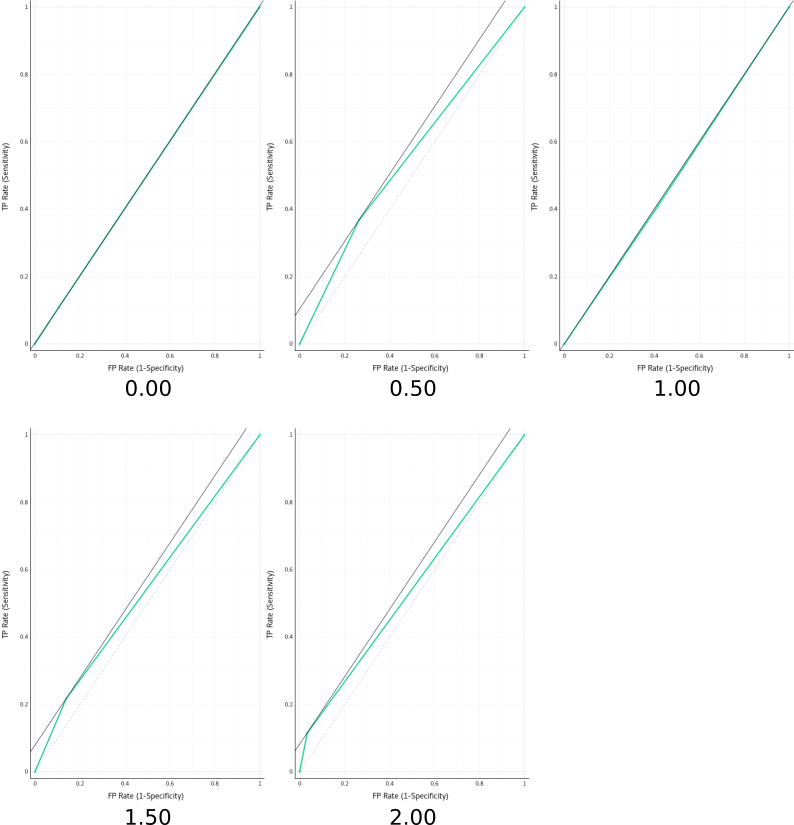
\includegraphics[scale=0.75]{figuras/roc.png}
\end{center}
\caption{Representação gráfica da Curva ROC para cada classe (0.00, 0.50, 1.00, 1.50 e 2.00) induzida no modelo AdaBoost.}
\label{fig:roc}
\end{figure}

O comportamento esperado para a curva, é que a mesma, se aproxime o máximo possível de 1 em cada classe. Entretanto a métrica se apresenta como uma reta nas classes 0.00 e 1.00, nas demais classes tende sutilmente a 1. Conclui-se que a predição das classes 0.00 e 1.00 nos testes estão ocorrendo de forma aleatório pelo classificador.

Por fim a tabela de contingência ou matriz de confusão, que através da discriminação dos erros ou acertos preditos para cada classe demonstra o desempenho do classificador, uma das métricas mais eficiente de se analisar um classificador. 

A Tabela ~\ref{tab:matrix_confusion} exibe ao longo da diagonal em tons de cinza as decisões corretas: número de verdadeiros positivos TP e verdadeiros negativos TN; já os elementos fora dessa diagonal representam os erros cometidos: número de falsos positivos FP e falsos negativos FN. É notável que o valor ideal fora da diagonal seja sempre igual a 0.  

\begin{table}[H]
\centering
\begin{tabular}{cc|c|c|c|c|c|c|}
\cline{3-8}
 &  & \multicolumn{6}{c|}{\textbf{Predição}} \\ \cline{3-8} 
 &  & \textbf{0.00} & \textbf{0.50} & \textbf{1.00} & \textbf{1.50} & \textbf{2.00} & $\sum_{}$  \\ \hline
\multicolumn{1}{|c|}{} & \textbf{0.00} & \cellcolor[HTML]{C0C0C0}4 & 18 & 13 & 2 & 0 & \textbf{37} \\ \cline{2-8} 
\multicolumn{1}{|c|}{} & \textbf{0.50} & 13 & \cellcolor[HTML]{C0C0C0}42 & 44 & 14 & 1 & \textbf{114} \\ \cline{2-8} 
\multicolumn{1}{|c|}{} & \textbf{1.00} & 18 & 51 & \cellcolor[HTML]{C0C0C0}78 & 32 & 11 & \textbf{190} \\ \cline{2-8} 
\multicolumn{1}{|c|}{} & \textbf{1.50} & 7 & 14 & 31 & \cellcolor[HTML]{C0C0C0}15 & 2 & \textbf{69} \\ \cline{2-8} 
\multicolumn{1}{|c|}{} & \textbf{2.00} & 4 & 2 & 14 & 3 & \cellcolor[HTML]{C0C0C0}3 & \textbf{26} \\ \cline{2-8} 
\multicolumn{1}{|c|}{\multirow{-6}{*}{\rot{Atual}}} & $\sum_{}$ & \textbf{46} & \textbf{127} & \textbf{180} & \textbf{66} & \textbf{17} & \textbf{436} \\ \hline
\end{tabular}
\caption{Tabela de contingência ou Matriz de confusão resultante da indução do classificador AdaBoost.}
\label{tab:matrix_confusion}
\end{table}

\subsection{Considerações Finais}

E notável que adversidade de classes desbalanceadas influenciou consideravelmente nos resultados preliminares.  A próxima etapa deste estudo merece destaque em uma seção exclusiva para discussão do tema e a análise dos principais métodos na literatura para balanceamento de classes.

As dificuldades observadas no estudo do problema proposto motivam melhorias e o surgimento de novas estratégias pra a continuidade do trabalho. 

% Os primeiros experimentos realizados na predição, ilustrado no Gráfico abaixo, demonstraram uma taxa de 30\% de acerto na predição da primeira competência exigida em um texto de redação, de uma amostra de 100 redações. 

% A análise gráfica do resultado experimental demonstra que a predição do modelo está em uma faixa especifica de 0.5 a 1.5, ou seja, a indução do modelo deve ser repetida até o mesmo se tornar genérico.

% \pgfplotstableread[col sep=semicolon]{data/adaboost_competence_1.dat}\data
% \begin{figure}[H]
% \begin{center}

% \begin{tikzpicture}
%     \begin{axis}[
%         title=Demonstrar domínio da norma padrão da língua escrita. (1ªCompetência ),
%         width=\textwidth,
%         ymin=0,
%         ytick={0,0.5,1.0,1.5,2.0},
%         ylabel=Pontuação,
%         xtick=data,
%         xticklabel style={rotate=90,anchor=east},
%         xticklabels from table={\data}{title},
%         legend style={ legend columns=-1},
%         enlarge x limits=0.01
%         ]
%         \addplot table[x=id, y=comp1] {\data};
%         \addplot table[x=id, y=adaboost] {\data};
%         \legend{Profissional,AdaBoost}
%     \end{axis}
% \end{tikzpicture}
% \end{center}
% \end{figure}

